\documentclass[12pt]{article}
\usepackage[slovene]{babel}
\usepackage[utf8]{inputenc}
\usepackage{makeidx}
\usepackage{pifont}
\usepackage{listings}  
\usepackage{hyperref}  
\usepackage{graphicx}
\usepackage[margin=0.8in]{geometry}
\usepackage[xindy,toc,acronym]{glossaries}

\graphicspath{{diagrami/}}

\let\stdsection\section
\renewcommand\section{\newpage\stdsection}

\title{Veriga prodajaln enolončnic}
\author{Andraž Brodnik, Domen Kožar}
\begin{document}

% quotes fix

\maketitle

\tableofcontents


\section{Uvod}


Reševali bomo problem prodajaln enoloncnic. 

Torej imamo več prodajaln enolončnic na večih lokacijah.

Prodajamo enolončnice (preprosta jed iz več vrst živil, pripravljena v enem loncu). Prodajalne imajo v ponudbi več enolončnic.

\subsection{Poslovalnica}

Poslovalnica je prodajalna je na neki lokaciji. V svoji ponudbi ima enolončnice. V ponudbi je vec enoloncnic, ni pa nujno, da so na voljo vse, ki jih zna nasa družba skuhati.

Prodajalna ima ime, ulico, hišno številko, poštno številko.

\subsection{Enolončnice}

Enolončnice so sestavljene iz več sestavin. Ter imajo ime in ceno, ki je enaka za vse prodajalne.


\subsection{Sestavine}

Sestavine so del enolončnice, imajo ime ter svojega dobavitelja. Dobavitelj je lahko samo eno podjetje.

\subsection{Dobavitelji}

Dobavitelji so podjetja z imenom. En dobavitelj lahko dobavlja več sestavin.

\subsection{Stranke}

Stranke lahko naročajo enoloncnice, preko naročila.
Imajo ime in priimek.

\subsection{Naročila}

Stranke izdajo naročilo. V naročilu je lahko več različnih enolončnic. Vendar lahko stranka naroči le eno enolončnico določenega tipa.


\section{Klasične diagramske tehnike}

\subsection{Entitetni diagram}

\begin{figure}[htb]
\begin{center}
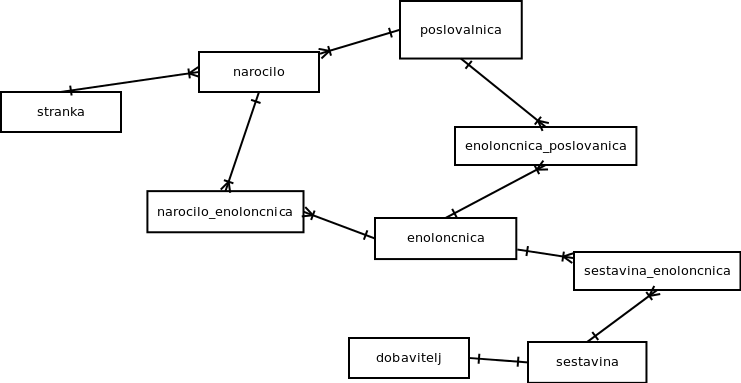
\includegraphics[scale=0.5]{entitetni.png}
\end{center}
\caption{Entitetni diagram}
\label{entitetni}
\end{figure}


Entitetni diagram nam opisuje relacije med tabelami v relacijski bazi. 

Kot vidimo imamo 3 tabele, ki nam "many to many" relacije razbije na "one to many". To so tabele enoloncnica\_poslovalnica, narocilo\_enoloncnica ter sestavina\_enoloncnica.

Prisotni so tudi objekti, ki smo jih opisali zgoraj.

% Pri tem velja upozoriti, da je "narocilo\_enoloncnica" rahlo posebna tabela, saj poleg informacije takero enoloncnica je v narocilu nosi tudi informacija, koliko teh enolocnic je v tem narocilu.  Ne velja


\newpage

\subsection{Funkcijska dekompozicija}

\begin{figure}[htb]
\begin{center}
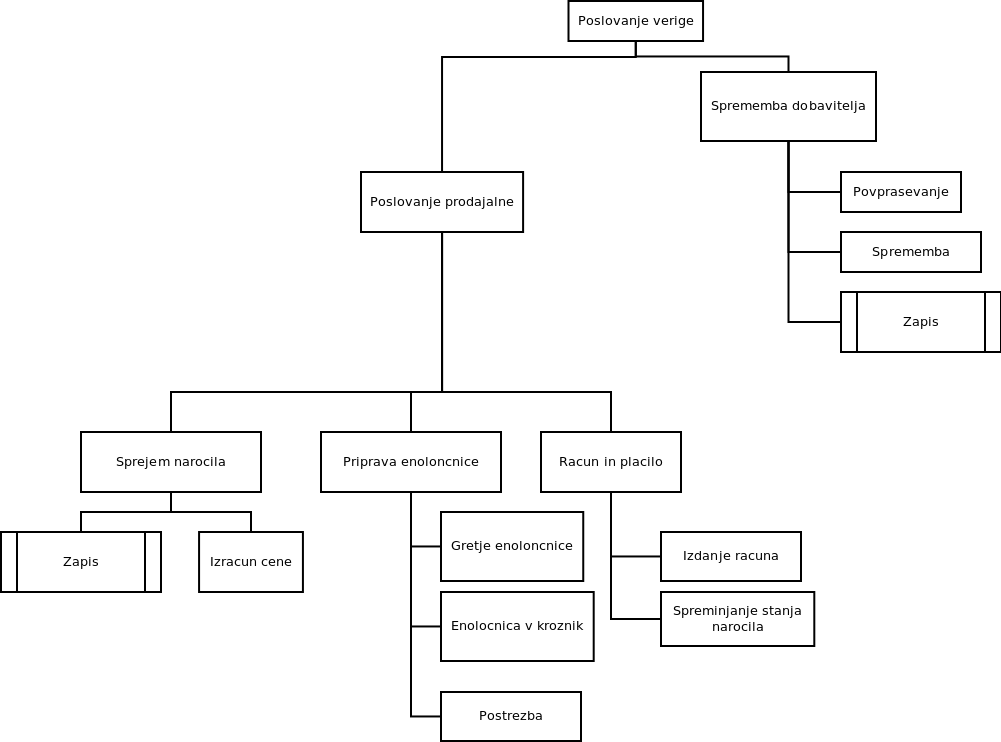
\includegraphics[scale=0.5]{funkcijska_dekompozicija.png}
\end{center}
\caption{Funkcijska dekompozicija}
\label{funkcijska_dekompozicija}
\end{figure}

Opisane so funkcije v našem poslovanju, zaradi preglednosti tabele smo se odpovedali razšeljivim in skrčljivim funkcijam.
Funkcijska dekompozicija je sestavljena iz funkcij in podfunkcij, to lahko razberemo iz drevesne strukture.

Naj opozorimo bralca na posebno funkcijo Zapis. Ta se ponavlja večkrat to je skupna funkcija.


\newpage

\subsection{Procesni diagram}

\begin{figure}[htb]
\begin{center}
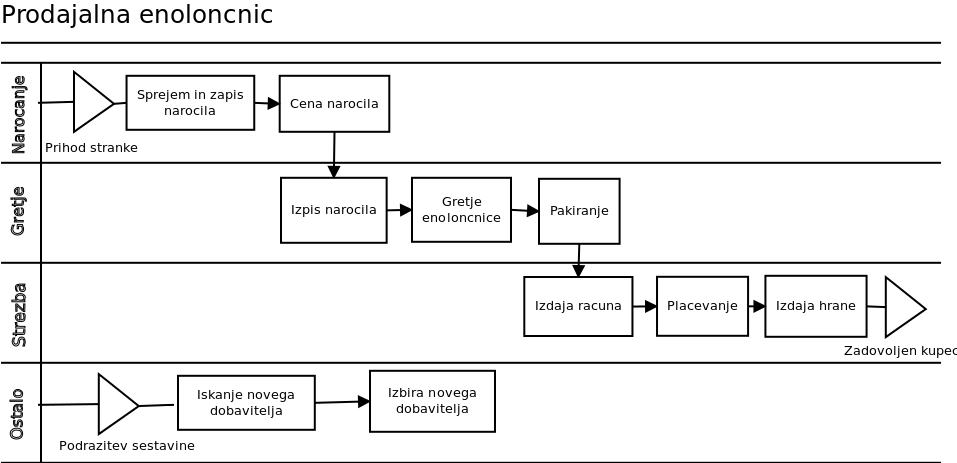
\includegraphics[scale=0.5]{procesni.png}
\end{center}
\caption{Procesni diagram}
\label{procesni}
\end{figure}

Prikazan je procesni diagram, ki nam govori o interakcijah med funkcijami. Na nasem grafu nastopa sprožilec (Stranka). 

Opisali smo standartni proces, ki ga pričakujemo v nasem delovnem procesu.
Dodali smo tudi proces, spreminjanja dobavitelja.

\newpage

\subsection{Diagram toka podatkov}

\begin{figure}[htb]
\begin{center}
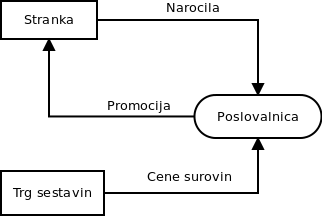
\includegraphics[scale=0.5]{toka_podatkov.png}
\end{center}
\caption{Diagram toka podatkov}
\label{toka_podatkov}
\end{figure}

Tok podatkov, ki je pomemben za delovanje naše družbe je prikazan na zgornjem grafu. Najbolj pomemben del je tok podatkov z Stranko. Od nje pridobivamo naročila, kar pomeni da lahko optimiziramo tudi jedilnik. Stranko informiramo z promocijo.
Preprostimi tablami pred poslovalnicami.

Trg sestavin vpliva na izbiro dobavitelja.

\newpage

\section{UML}

\subsection{Diagram primerov uporabe}

\begin{figure}[htb]
\begin{center}
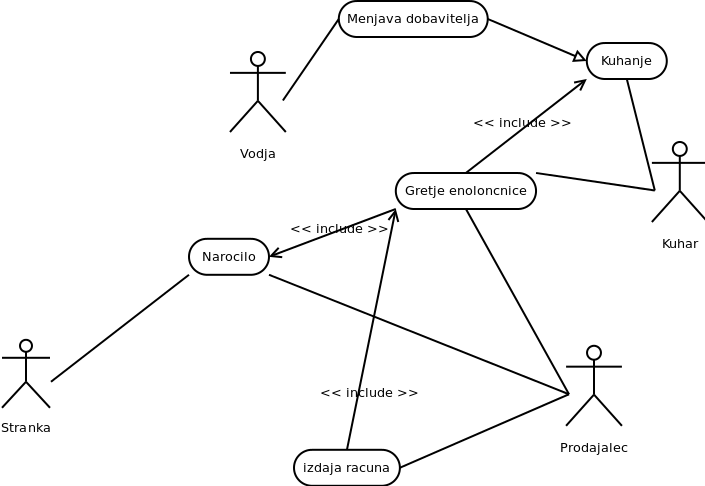
\includegraphics[scale=0.5]{primer_uporabe.png}
\end{center}
\caption{Diagram primerov uporabe}
\label{primer_uporabe}
\end{figure}

Na diagramu smo prikazali odvisnosti resitve primerov uporabe. Kot je razvidno je, da ne moremo greti enolončnice, če nimamo naročila oz enoločnica ni skuhana. Račun izdamo ko je enolončnica pogreta. 

Dodamo še kuharja in kuhanje, da lahko dodamo spremembo dobaviteljev.

\newpage

\subsection{Diagram sodelovanja}

\begin{figure}[htb]
\begin{center}
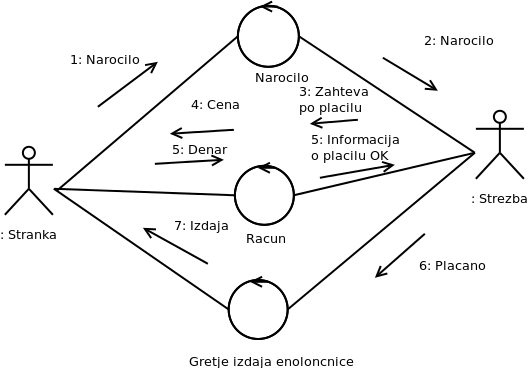
\includegraphics[scale=0.5]{sodelovanja.png}
\end{center}
\caption{Diagram sodelovanja}
\label{sodelovanja}
\end{figure}

Tukaj imamo prikazana sodelovanje med akterji ter sporočila, ki so našteta po vrsti izvajanja.

\newpage

\subsection{Diagram stanj}

\begin{figure}[htb]
\begin{center}
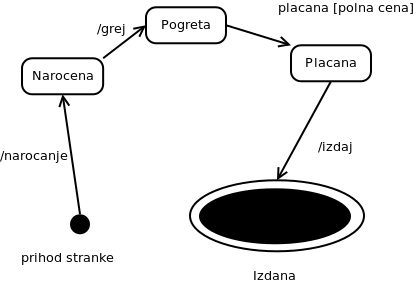
\includegraphics[scale=0.5]{stanj.png}
\end{center}
\caption{Diagram stanj}
\label{stanj}
\end{figure}

Na levi strani spodaj imamo začetno stanje, na desni strani spodaj pa končno stanje. Ko je enoločnica naročena,
jo pogrejemo preide v stanje pogreta, ko jo stranka plača, ji lahko izdamo.



\newpage

\subsection{Diagram aktivnosti}

%\begin{figure}[htb]
%\begin{center}
%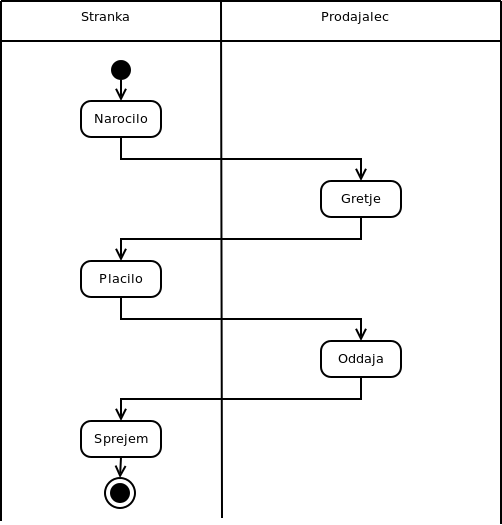
\includegraphics[scale=0.5]{aktivnosti.png}
%\end{center}
%\caption{Diagram aktivnosti}
%\label{aktivnosti}
%\end{figure}



\newpage

\section{SQL}


\end{document}
